
\documentclass[british,11pt,a4paper]{article}
\usepackage[british]{babel}
\usepackage[margin=1in, bottom=0.75in, top=0.75in, footskip=0.25in]{geometry}
\usepackage[titletoc]{appendix}
\usepackage{fancyhdr}
\usepackage{mathtools}
\usepackage[numbers]{natbib}
\usepackage{pgfplotstable,filecontents}
\usepackage{hyperref}
\usepackage{booktabs}
\usepackage{wrapfig}
\usepackage{listings}
\usepackage{color}
\usepackage{graphicx}
\usepackage{siunitx}
\usepackage[parfill]{parskip}
\usepackage{tikz} % To generate the plot from csv
\usepackage{pgfplots}
\usepackage[normalem]{ulem}
\usepackage{longtable}
\useunder{\uline}{\ul}{}

\usepgfplotslibrary{statistics}

\pgfplotsset{compat=newest} % Allows to place the legend below plot
\usepgfplotslibrary{units} % Allows to enter the units nicely

\graphicspath{ {images/} }

\setcounter{secnumdepth}{2}
\setcounter{tocdepth}{2}
\renewcommand{\arraystretch}{1.2}
\renewcommand\thesection{\arabic{section}}
\renewcommand\thesubsection{\roman{subsection}.}
\renewcommand\thesubsubsection{}
\newcommand*{\Appendixautorefname}{appendix}
\pagestyle{fancy}
\fancyhf{}
\renewcommand{\headrulewidth}{0pt}
\lfoot{Exam no: Y0076159}
\cfoot{\thepage}
\lstset{
  columns=fixed,
  breaklines=true,
  basicstyle=\ttfamily\footnotesize
  }

\usepackage[nottoc]{tocbibind}
\usepackage{csvsimple}

\begin{document}
\title{PSEC Open Assessment}
\author{Exam no: Y0076159}
\date{\today}
\maketitle
\tableofcontents
\clearpage

\section{Question 1 - Security risk management assessment}
\subsection{Purpose and scope}

\subsection{Security risks}
\subsubsection{Identification}
\subsubsection{Analysis}
\subsubsection{Evaluation}
\subsubsection{Treatment}

\clearpage


\section{Question 2 - Bulk guessing tool}

\subsubsection{Bulk guessing}
Bulk guessing, as described by \citet{Florencio2007-yp}, is the action of attempting of accessing an authentication-protected account on a system by attempting to guess the password for a large number of accounts, using a large number of guess passwords (which are either randomly generated or randomly sampled from a dictionary). As password policies set in place by institutions aim to deter attackers from guessing a single password, the act of simultaneously breaking millions of accounts can yield a successful guesses on a few different accounts. The tool designed for this project aims to demonstrates the expected success rate of a bulk guessing algorithm using an attack dictionary, which is evaluated against a set of statistically common passwords from \citet{rockyoupasswords}.

\subsection{Design \& Implementation}
The tool is implemented in python 2.7.6, and can be ran using the command \lstinline{python main.py M N1 N2} where M is the number of guesses, N1 is the minimum password length and N2 is the exact password length. This will print an output detailing the number of correct guesses for each authentication method. Additional options can be passed to the tool: \lstinline{-its n} runs the program n times, and \lstinline{--save_file} saves the results of each run to a datafile.


\subsubsection{Data handling}
Two classes are used to handle data sources. AttackPasswords is used to retrieve the passwords used in bulk guessing, and pre-filters them according to arguments N1 and N2. An error check is put into place to ensure the lists of passwords/passcodes are not empty, as this would be an unusable attack vector for bulk guessing. The class also implements $pick\_password\_passcode()$ which returns a (password, passcode) tuple randomly selected from the list of 500 passwords.

The distribution of common passwords is handled by the VictimPasswords class, which conducts some optimisation to improve the performance of the attack at the cost of memory usage. This is achieved by retrieving each password and frequency, and appending it repeatedly to a large list in proportion to it's frequency. This allows us to sample the distribution of passwords according to their weight, but by using a $O(1)$ complexity by generating a random float in $\{0,1\}$ and retrieving the value at that index of the array. This accrues a significant memory usage, as a large number of duplicate passwords are stored, but significantly reduces the complexity of the algorithm which would otherwise require $O(n)$ to randomly select an adequate password. The memory usage was later minimised using a de-facto pointer, where each value is wrapped in an object of class $Value$, and the same instance of the object is stored at multiple indices of the array. As they point to the same value, this avoids duplicating the value in memory, at the cost of memory usage to define the class instance and pointer.

\subsubsection{Password comparison}
Two methods implement the password authentication: $match(victim, guess)$ randomly picks 3 different integers in the range of the victim's password, and compares the characters at those indices with the guess password. This includes error catching for the cases where the victim selects a password larger than the policy but the bulk guessing randomly picks a shorter one, which could result in an IndexError, or for a blank password (which has no indices). A second method, $matchfull(password, guess)$ provides a simple string equality check to validate complete passwords.
 

\subsection{Results \& Analysis}
\subsubsection{Comparison of authentication methods}
\label{subsec:authentication_methods}
Our implementation was ran 150 times for $n1, n2 \in \{6,7,8\}$, resulting in data with extremely precise confidence intervals as seen in \autoref{fig:approach_comparison}. The results demonstrate that for all combinations of password and passcode length, the second authentication system is more vulnerable to bulk guessing than the first. This is found to be statistically significant across all password/passcode combinations, as visible in \autoref{app:significant_stats} where a two-tailed Mann-Whitney test was used to show that $p<.01$ between each algorithm for all equivalent password/passcode policies. Partial password authentication is therefore between 1.91 and 3.5 times more likely to be randomly guessed, depending on the password/passcode policies chosen (minimum ratio at password/passcode of 8/7, and maximum ratio at 6/6).

These observations are most likely due to two effects. Firstly, we should state that every successful password guess in the full password system will be a successful guess in system B (with partial password matching), as the indices compared in the partial password system form a subset of the indices compared to the full password. Secondly, full passwords require the victim and attacker passwords to have the same length; this is not always the case, as the policy sets only a minimum bound on the password length, leading to mis-matched password lengths. This would cause the guess to fail for a full password, but not a partial password (assuming the characters stated indices matched). Finally, there is a significant number of password collisions at various indices which allow a larger number of guess passwords to correctly guess a victim's password. 

This was verified using a brute force script (see \autoref{app:bruteforce}, which evaluated every combination of guess and victim password using either a full match or every combination of 3 indices within the password's length. This resulted in the data seen in \autoref{fig:collision_prob}: as we can see, the index-based authentication system (Syfull) results in a significantly higher probability of guessing a password in a bulk attack. Whilst our dataset may exaggerate this effect, it is reasonable to assume that whilst a single password can only be fully guessed by a copy of itself, it could be partially guessed by a larger number of passwords which happen to match it's characters in stated indices, and it is therefore more likely that one of these passwords will be selected at random as there are a larger number of them. 
\begin{figure}
	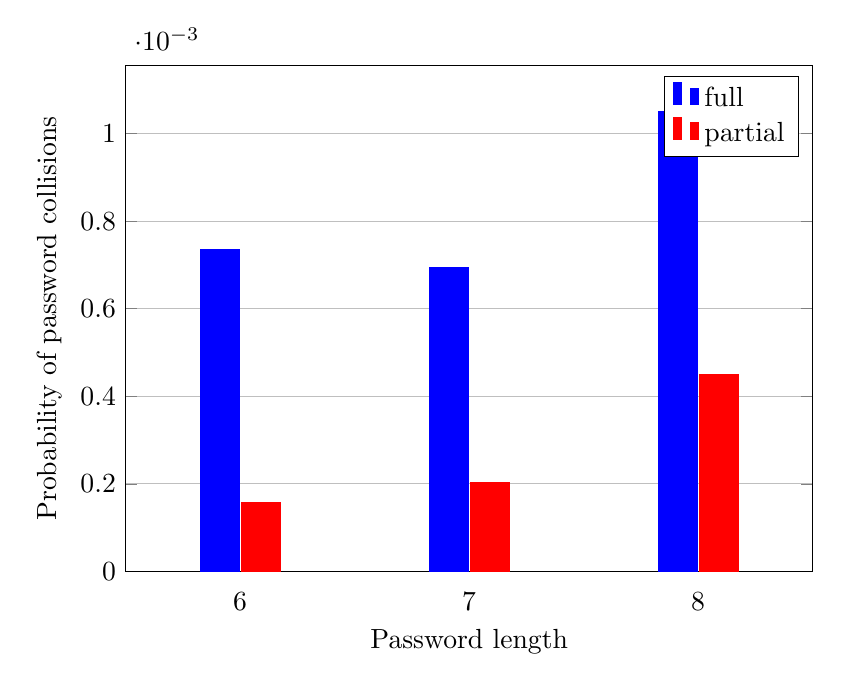
\begin{tikzpicture}
	    \begin{axis}[
	        width  = 0.85*\textwidth,
	        height = 8cm,
	        major x tick style = transparent,
	        ybar=2*\pgflinewidth,
	        bar width=14pt,
	        ymajorgrids = true,
	        ylabel = {Probability of password collisions},
	        symbolic x coords={6, 7, 8},
	        xtick = data,
	        xlabel = Password length,
	        enlarge x limits=0.25,
	        ymin=0,
	        legend cell align=left,
	    ]
	        \addplot[style={blue,fill=blue,mark=none}]
	            coordinates {(6, 7.36E-04) (7,6.94E-04) (8,1.05E-03)};

	        \addplot[style={red,fill=red,mark=none}]
	             coordinates {(6,1.56E-04) (7,2.02E-04) (8,4.50E-04)};
	        \legend{full, partial}
	    \end{axis}
	\end{tikzpicture}
	\caption{Probability of guessing a password using character sampled authentication (Syfull) and full password authentication (Sypart).}
	\label{fig:collision_prob}
\end{figure}

\subsubsection{Effects of password policy}
The password policies have similar effects on both algorithms: increasing the passcode length decreases the number of successful guesses, whilst increasing the password length increases the number of successful guesses. The latter observation is at first surprising: as a larger password/passcode length would allow for a larger number of permutations, one would expect the number of successful guesses to decrease as the password's length increases due to a decreased probability. As this effect is observed for both forms of authentication, we can deduce it is not caused by the the difference in these systems (i.e: using 3 characters instead of a full password to establish validity). Further analysis of the data show that the number of valid passwords in our dataset decreases as we increase the minimum password length; for both our 500 attack passwords and the RockYou password distribution \cite{rockyoupasswords}. As visible in \autoref{fig:passwords_length}, this leads to a smaller number of possible guess password/account password combinations ($4 \times 10^6 $ for  passwords  of length $<= 8$, $9 \times 10^7$ for passwords of length $<= 6$). This results in a larger number of correct guesses for a fixed sample size, causing the effect seen in \autoref{fig:approach_comparison}. The effect does not occur for passcodes however, as the number of passcodes in \cite{rockyoupasswords} for each policy length remains roughly constant (89,595 for n=6 to 55,803 for n=8). 

We could therefore state that increasing the minimum password length policy can cause user accounts which utilise dictionary passwords to be more vulnerable to bulk guessing, as the the set of possible passwords is reduced as the minimum size increases.



% TODO proof read

%Papers to look at
% https://www.usenix.org/legacy/event/hotsec07/tech/full_papers/florencio/florencio.pdf
% http://www.ijafrc.org/Volumn1/Vol_issue12/12.pdf
% https://www.ece.cmu.edu/~lbauer/papers/2016/usenixsec2016-neural-passwords.pdf

%Partial passwords
%http://groups.inf.ed.ac.uk/security/passwords/pps.pdf
% http://translate.google.pl/translate?sl=pl&tl=en&js=n&prev=_t&hl=pl&ie=UTF-8&layout=2&eotf=1&u=http://wampir.mroczna-zaloga.org/archives/235-o-haslach-maskowanych.html

\begin{figure}
	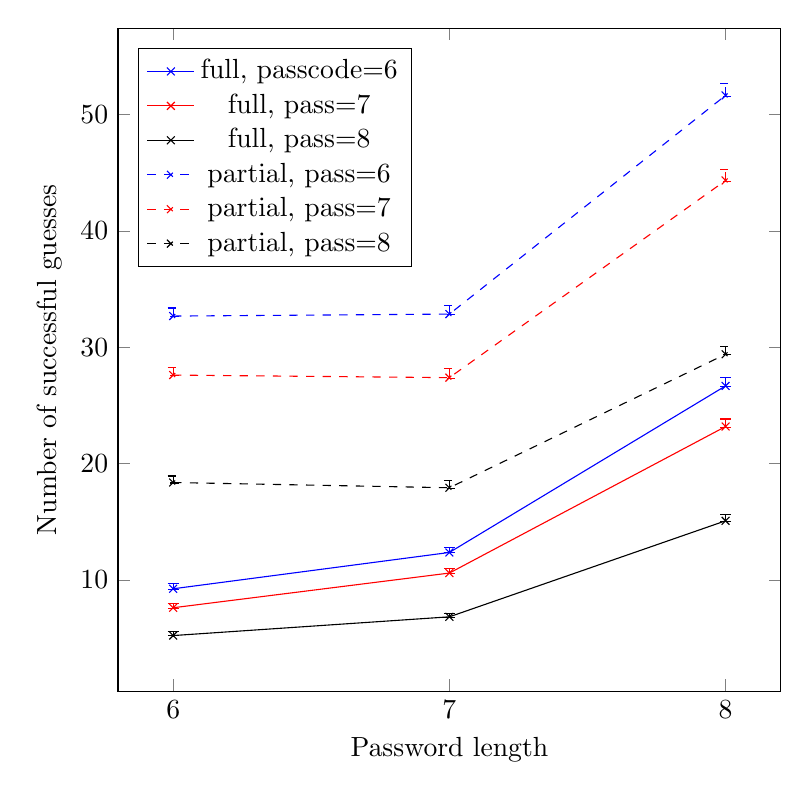
\begin{tikzpicture}
	    \begin{axis}[
	    	height=10cm,
	    	width=10cm,
	    	xtick={6,7,8},
	        xlabel=Password length,
	        ylabel=Number of successful guesses,
	        legend pos=north west
	    ]
	    \addplot[
	        mark=x,
	        blue,
	        error bars/.cd, y dir=both, y explicit,
	    ] plot coordinates {
	        (6,9.25)   -=(0,0.033) += (0,0.438)
	        (7,12.37)  -=(0,0.034) += (0,0.450)
	        (8,26.68)  -=(0,0.058) += (0,0.759)
	    };
	    \addlegendentry{full, passcode=6}

	    \addplot[
	        mark=x,
	        red,
	        error bars/.cd, y dir=both, y explicit,
	    ] plot coordinates {
	        (6,7.62)  -= (0,0.030) += (0,0.398)
	        (7,10.60) -= (0,0.030) += (0,0.397)
	        (8,23.19) -= (0,0.049) += (0,0.645)
	    };
	    \addlegendentry{full, pass=7}    

	    \addplot[
	        mark=x,
	        error bars/.cd, y dir=both, y explicit,
	    ] plot coordinates {
	        (6,5.23)  -= (0,0.025) += (0,0.329)
	        (7,6.84)  -= (0,0.024) += (0,0.319)
	        (8,15.09) -= (0,0.039) += (0,0.504)
	    };
	    \addlegendentry{full, pass=8}

	    \addplot[
	        mark=x,
	        blue,
	        dashed,
	        error bars/.cd, y dir=both, y explicit,
	    ] plot coordinates {
	        (6,32.68)  -=(0,0.053) += (0,0.695)
	        (7,32.85)  -=(0,0.058) += (0,0.753)
	        (8,51.64)  -=(0,0.078) += (0,1.026)
	    };
	    \addlegendentry{partial, pass=6}

	    \addplot[
	        mark=x,
	        red,
	        dashed,
	        error bars/.cd, y dir=both, y explicit,
	    ] plot coordinates {
	        (6,27.61) -= (0,0.053) += (0,0.690)
	        (7,27.39) -= (0,0.057) += (0,0.749)
	        (8,44.33) -= (0,0.070) += (0,0.921)
	    };
	    \addlegendentry{partial, pass=7}    

	    \addplot[
	        mark=x,
	        dashed,
	        error bars/.cd, y dir=both, y explicit,
	    ] plot coordinates {
	        (6,18.38)  -= (0,0.043) += (0,0.559)
	        (7,17.93)  -= (0,0.046) += (0,0.599)
	        (8,29.40)  -= (0,0.049) += (0,0.645)
	    };
	    \addlegendentry{partial, pass=8}

	    \end{axis}
	\end{tikzpicture}
	\caption{Mean number of successful guesses from ($50 \times 10^6 $) attempts using varying passcode length}
	\label{fig:approach_comparison}
\end{figure}

\begin{figure}
	\begin{tikzpicture}
	    \begin{axis}[ybar, xtick = {6,7,8}, xlabel = Minimum password length, ylabel = Number of valid account passwords in \cite{rockyoupasswords}]
		\addplot table [
		        col sep=comma,
		        x=pass_size,
		        y=num_pass,
		    ] {data/password_count.csv};
	    \end{axis}	    
	    \begin{axis}[
	    	axis y line*=right,
    		axis x line=none, 
    		ylabel = Number of valid attack passwords out of 500]
		\addplot table [
		        col sep=comma,
		        x=pass_size,
		        y=guess_pass,
		    ] {data/password_count.csv};
	    \end{axis}
	\end{tikzpicture}
	\caption{Count of valid passwords in \cite{rockyoupasswords} for each password policy}
	\label{fig:passwords_length}
\end{figure}


\subsection{Application of authentication systems}
These two authentication systems are both viable systems, but differ in their ability to protect users from various forms of attack. As we have previously demonstrated in \autoref{subsec:authentication_methods}, partial password authentication is significantly more vulnerable to bulk guessing than a full password authentication (as discussed by \citet{Aspinall2013-sh}). This observation is restricted to the case where user-chosen passwords offer a high degree of collision with our attack dictionary (as demonstrated in \autoref{fig:collision_prob}); using system generated random passwords would likely reduce the difference in vulnerability to some extent, although partial guessing will still be more vulnerable due to the multitude of possible solutions to the challenge (the set of password characters requested by the authentication system). We should also note that the use of random passwords could result in more frequent password recovery emails, shifting the security vulnerability from the login system to the password reset system. The vulnerability can however be accentuated through the use of projection dictionaries, which would select the most common 3-tuple of characters at the challenge's stated indeces. We can therefore deduce that partial password authentication is more vulnerable than full password authentication when considering bulk guessing as the sole attack vector.

Within a real-world scenario, an attacker could easily improve his success rate by using additional tools. This represents one of the major benefits of partial passwords: a recorded session may not be sufficient to provide authentication, assuming that the challenge indices change between the victim and attacker's login attempts; in contrast, a full password authentication would allow the entire password to be recorded, allowing the attack to break that security with ease. Mitigating the effectiveness of keyloggers is therefore the primary use of partial passwords. \citet{Aspinall2013-sh} demonstrates that keyloggers can nevertheless greatly improve the success rate against partial passwords: a 25\% success rate was observed using dictionary attack with a single recording (vs 5.5\% without keylogger), and 81\% using 4 recordings. These were undertaken using a slightly different password policy: 36 alphanumeric characters (excluding symbols), a password length of 8, a 3 character challenge and a 10 attempt lockout. It remains applicable to our given case study, thereby demonstrated that the presence of a keylogger on a system for an extended period of time can greatly mitigate the benefit of partial passwords. We should nevertheless consider that partial passwords would provide security against shoulder-surfing attacks, where the attacker observes the victim logging in, as it is unlikely that the attacker will observe as many logins in person than using a discrete keylogger. 

Therefore, we can state that within the attack vector of password guessing through either bulk attack and/or keylogging, full and partial password authentication mitigate different attack vectors: partial passwords are more vulnerable to bulk guessing, but are more resistant to keylogging attacks, whilst full passwords are the opposite. Combining the two approaches may give some common benefit, as demonstrated by Lloyds Bank's system; this would complicate the attack by requiring both keylogging and bulk guessing (in either order) to guess the full password and partial passcode. In contrast, Virgin's authentication system could be cracked solely using bulk guessing, which could be optimised by a key logger.

A further problem of partial passwords would include storing the password digest on a server side. While this is straightforward for full passwords, which can be fully salted and hashed to form the digest, partial passwords would require the use of a shared secret \cite{smartarchitect}, or storing multiple digests of every m-letter combination (where m is the size of the challenge) \cite{smartarchitect}. The latter solution would result in a large number of digests, which could be a source of vulnerability if a large sample of them were collected. 





\subsection{Counter-measures}
Counter-measures to bulk guessing attacks would be two-fold: system side policies should reduce the success rate of bulk attacks to an acceptable threshold, and client side security must be put in place to reduce the vulnerability to keyloggers, as these are capable of greatly negating client side security. We will address these in the following two sections.

\subsubsection{Server side policies}
We can reduce the number of attempts that the attacker can make on a system, by imposing a rate limit on the number of authentication attempts from a host within a given timespan \cite{Florencio2007-yp}, or by imposing a 3-strike rule which would require the users to reset the password via a secure channel \cite{Florencio2007-yp}. These would mitigate the attacker's ability to conduct the attack by requiring either a larger number of attack sources (i.e: a botnet), and access to a large number of userID's with which to conduct the attack (as these will quickly be locked out by unsuccessful attempts). This could be a probabilistically (expected number of cracked accounts before all accounts are locked down $\approx$ 0) secure for smaller institutions, with hundreds rather than millions of accounts \cite{Florencio2007-yp}, but not wholly sufficient for large institutions. 

The latter factor can be greatly enlarged by increasing the userID size: this would greatly increase the credential space, requiring the attacker to either gather these credentials prior to the bulk guessing, or significantly increasing the complexity of the attack by forcing a userID to be randomly guessed \cite{Kosamkar_undated-ik}. The complexity could be further increased through the use of obfuscated errors to unsuccessful logins, which do not state whether the userID or password were incorrect, forcing the search to continue through a large credential space. Finally, the use of an Automated Turing Test, such as Google's AI-based captcha \cite{noauthor_undated-lk}, could cause a fraction of logins to be evaluated, as there is only a small probability of randomly guessing an ATT (by design). Placing this challenge in between the login attempt and response would prevent the attacker from viewing the result of a majority of attempts, thereby greatly increasing the complexity of the attack \cite{Alsaleh2012-ek}. \citet{Alsaleh2012-ek} demonstrates a comprehensive ATT protocol named PGRP (Password Guessing Resistant Protocol) which is effective at significantly reducing the effectiveness of bulk guessing.

Password and passcode policies could be maximised to increase the complexity of the attack, but \citet{Florencio2007-yp} has determined that the combined userID/password credential space is more significant in deterring bulk guessing attacks than just the password space. Forcing the use of randomly generated password/passcodes could fully mitigate the benefit of dictionary or projected dictionary attacks \cite{Kosamkar_undated-ik}, which would greatly increase the attack complexity (\citet{Aspinall2013-sh} demonstrates the performance of brute force over 8 character alphanumerical passwords to be 0.002 \% success rate, against 5.5\% using a projected dictionary).

We could expect these methods to greatly increase the complexity of the attack, forcing the attacker to utilise a very large botnet and a large number of user passwords to crack fewer accounts. This would allow smaller institutions to almost fully mitigate the threat of bulk guessing attacks, whilst larger institutions could maintain their effectiveness to an acceptably small level, or at least improve their detectability. We should note that these methods are only viable to prevent on-line attack: if the rate-limiting methods were bypassed (for example by cracking the database off-line), the userID/password combinations would be the only form of attack mitigation remaining.

\subsubsection{Client-side security}
Finally, as \citet{Aspinall2013-sh} has demonstrated the significance of recording successful authentications on the vulnerability of partial passwords, ensuring the client's machine is adequately protected from keyloggers or shoulder surfing is paramount to the security of the user's account. The use of anti-spyware or anti-virus programs could allow the detection, disabling or cleansing of keyloggers, mitigating the chance of recording authentications. Additional software-based security could include network monitors, which could detect the keylogger's attempt to send the data back to the attacker, or on-screen keyboards which changes the input system. Stronger security systems could utilise security tokens, which could be obtained from dedicated hardware (such as a credit card reader, or smart-phone application) to obtain a one-time password which would be difficult to guess. These would represent the only hindrance to the system's acceptability, as it would require more complexity to utilise than simple userID/password/passcode authentication system. 

\clearpage
\bibliographystyle{IEEEtranSN}
\bibliography{references}
\clearpage

\begin{appendices}
	\section{Main.py}\label{app:main}
	\lstinputlisting[language=Python]{../main.py}	
	\clearpage

	\section{Statistics}\label{app:extra_stats}
	\subsection{Compiled statistics}
	\begin{table}[h]
		\centering
		\begin{tabular}{|l|l|l|l|l|l|l|l|}
		\hline
		& & \multicolumn{6}{l|}{\textbf{Auth system and passcode length}} \\ \hline
		\textbf{Mean} & \textbf{Password len} & \textbf{full, 6} & \textbf{full, 7} & \textbf{full, 8} & \textbf{part, 6} & \textbf{part, 7} & \textbf{part, 8} \\ \hline
		 & 6 & 9.25 & 7.62 & 5.23 & 32.68 & 27.61 & 18.38 \\ \hline
		 & 7 & 12.37 & 10.60 & 6.84 & 32.85 & 27.39 & 17.93 \\ \hline
		 & 8 & 26.68 & 23.19 & 15.09 & 51.64 & 44.33 & 29.40 \\ \hline
		\textbf{Median} &  &  &  &  &  &  &  \\ \hline
		 & 6 & 9.00 & 7.00 & 5.00 & 33.00 & 28.00 & 18.00 \\ \hline
		 & 7 & 12.00 & 10.50 & 6.50 & 33.00 & 28.00 & 18.00 \\ \hline
		 & 8 & 27.00 & 23.00 & 15.00 & 52.00 & 44.50 & 29.00 \\ \hline
		\textbf{STD} &  &  &  &  &  &  &  \\ \hline
		 & 6 & 3.26 & 2.96 & 2.45 & 5.17 & 5.14 & 4.16 \\ \hline
		 & 7 & 3.35 & 2.95 & 2.38 & 5.61 & 5.58 & 4.46 \\ \hline
		 & 8 & 5.65 & 4.80 & 3.75 & 7.64 & 6.86 & 4.80 \\ \hline
		\textbf{Min} &  &  &  &  &  &  &  \\ \hline
		 & 6 & 2.00 & 2.00 & 1.00 & 21.00 & 16.00 & 9.00 \\ \hline
		 & 7 & 5.00 & 4.00 & 2.00 & 21.00 & 10.00 & 6.00 \\ \hline
		 & 8 & 12.00 & 11.00 & 3.00 & 32.00 & 27.00 & 20.00 \\ \hline
		\textbf{Max} &  &  &  &  &  &  &  \\ \hline
		 & 6 & 18.00 & 15.00 & 14.00 & 46.00 & 43.00 & 29.00 \\ \hline
		 & 7 & 21.00 & 20.00 & 13.00 & 48.00 & 43.00 & 31.00 \\ \hline
		 & 8 & 43.00 & 38.00 & 24.00 & 75.00 & 64.00 & 44.00 \\ \hline
		\textbf{0.1 confi.} &  &  &  &  &  &  &  \\ \hline
		 & 6 & 0.033 & 0.030 & 0.025 & 0.053 & 0.053 & 0.043 \\ \hline
		 & 7 & 0.034 & 0.030 & 0.024 & 0.058 & 0.057 & 0.046 \\ \hline
		 & 8 & 0.058 & 0.049 & 0.039 & 0.078 & 0.070 & 0.049 \\ \hline
		\textbf{0.9 confi.} &  &  &  &  &  &  &  \\ \hline
		 & 6 & 0.438 & 0.398 & 0.329 & 0.695 & 0.690 & 0.559 \\ \hline
		 & 7 & 0.450 & 0.397 & 0.319 & 0.753 & 0.749 & 0.599 \\ \hline
		 & 8 & 0.759 & 0.645 & 0.504 & 1.026 & 0.921 & 0.645 \\ \hline
		\end{tabular}
		\caption{Individual statistics for each authentication system and password/passcode length combination}
	\end{table}
	\clearpage

  	\subsection{Data significance}
  	\label{app:significant_stats}
  	The following table details the results of statistical tests between each authentication system using equivalent password/passcode length policies.
  	\begin{table}[h]
	\centering
	\begin{tabular}{|l|l|l|l|l|}
	\hline
	\textbf{Password/Passcode length} & \textbf{full median} & \textbf{part median} & \textbf{Mann whitney Z-score} & \textbf{p value} \\ \hline
	6,6 & 9 & 33 & -14.974 & p\textless0.01 \\ \hline
	6,7 & 7 & 27.5 & -14.974 & p\textless0.01 \\ \hline
	6,8 & 5 & 18 & -15.100 & p\textless0.01 \\ \hline
	7,6 & 12 & 33 & -14.974 & p\textless0.01 \\ \hline
	7,7 & 10.5 & 28 & -14.793 & p\textless0.01 \\ \hline
	7,8 & 6.5 & 18 & -14.596 & p\textless0.01 \\ \hline
	8,6 & 27 & 52 & -14.898 & p\textless0.01 \\ \hline
	8,7 & 23 & 44.5 & -14.801 & p\textless0.01 \\ \hline
	8,8 & 15 & 29 & -14.794 & p\textless0.01 \\ \hline
	\end{tabular}
	\caption{Statistical tests between authentication systems for equivalent password/passcode length}
	\label{tab:significance}
	\end{table}

	\subsection{Sample of raw data}
	\label{app:raw_data}
	\begin{longtable}{|l|l|l|l|l|l|l|l|l|l|l|l|l|l|l|l|l|l|}
	\hline
	\multicolumn{18}{|l|}{\textbf{Password/Passcode policy in format N1/N2, full $\rightarrow$ full, part $\rightarrow$ partial}} \\ \hline
	\multicolumn{2}{|l|}{\textbf{6,6}} & \multicolumn{2}{l|}{\textbf{6,7}} & \multicolumn{2}{l|}{\textbf{6,8}} & \multicolumn{2}{l|}{\textbf{7,6}} & \multicolumn{2}{l|}{\textbf{7,7}} & \multicolumn{2}{l|}{\textbf{7,8}} & \multicolumn{2}{l|}{\textbf{8,6}} & \multicolumn{2}{l|}{\textbf{8,7}} & \multicolumn{2}{l|}{\textbf{8,8}} \\ \hline
	full & part & full & part & full & part & full & part & full & part & full & part & full & part & full & part & full & part \\ \hline
	12 & 36 & 6 & 27 & 3 & 24 & 7 & 23 & 10 & 21 & 6 & 17 & 21 & 42 & 32 & 51 & 16 & 26 \\ \hline
	17 & 39 & 12 & 28 & 7 & 17 & 14 & 48 & 13 & 26 & 6 & 19 & 29 & 47 & 23 & 37 & 16 & 30 \\ \hline
	11 & 27 & 5 & 23 & 5 & 11 & 13 & 42 & 13 & 26 & 5 & 11 & 31 & 57 & 20 & 46 & 18 & 35 \\ \hline
	11 & 32 & 7 & 29 & 3 & 17 & 8 & 32 & 5 & 20 & 7 & 21 & 24 & 47 & 20 & 42 & 13 & 26 \\ \hline
	9 & 21 & 7 & 26 & 5 & 17 & 7 & 28 & 10 & 27 & 7 & 13 & 27 & 52 & 28 & 48 & 11 & 29 \\ \hline
	13 & 42 & 11 & 27 & 2 & 14 & 14 & 45 & 11 & 25 & 4 & 18 & 24 & 57 & 16 & 30 & 9 & 24 \\ \hline
	12 & 36 & 4 & 23 & 4 & 15 & 12 & 36 & 8 & 31 & 5 & 21 & 29 & 58 & 24 & 44 & 17 & 33 \\ \hline
	13 & 36 & 11 & 35 & 4 & 14 & 10 & 27 & 11 & 27 & 7 & 15 & 40 & 64 & 31 & 62 & 19 & 34 \\ \hline
	10 & 40 & 12 & 39 & 7 & 21 & 6 & 25 & 12 & 30 & 4 & 18 & 30 & 54 & 25 & 48 & 15 & 34 \\ \hline
	10 & 34 & 8 & 22 & 6 & 17 & 16 & 34 & 11 & 32 & 3 & 11 & 37 & 59 & 21 & 38 & 15 & 28 \\ \hline
	5 & 32 & 7 & 28 & 5 & 14 & 19 & 29 & 13 & 26 & 5 & 17 & 29 & 49 & 15 & 34 & 13 & 32 \\ \hline
	17 & 34 & 4 & 26 & 3 & 19 & 11 & 29 & 12 & 30 & 4 & 16 & 20 & 43 & 19 & 40 & 22 & 34 \\ \hline
	5 & 26 & 9 & 30 & 7 & 18 & 14 & 42 & 10 & 21 & 10 & 17 & 33 & 67 & 21 & 43 & 20 & 30 \\ \hline
	16 & 30 & 5 & 26 & 3 & 13 & 16 & 33 & 12 & 29 & 6 & 20 & 31 & 65 & 20 & 51 & 17 & 22 \\ \hline
	18 & 46 & 8 & 23 & 5 & 25 & 15 & 36 & 18 & 36 & 12 & 20 & 29 & 46 & 24 & 44 & 22 & 31 \\ \hline
	15 & 39 & 3 & 27 & 8 & 27 & 10 & 28 & 11 & 23 & 6 & 22 & 31 & 67 & 20 & 39 & 17 & 29 \\ \hline
	10 & 37 & 7 & 29 & 5 & 21 & 17 & 43 & 11 & 28 & 6 & 11 & 19 & 47 & 27 & 48 & 19 & 35 \\ \hline
	8 & 30 & 5 & 21 & 3 & 13 & 11 & 31 & 11 & 24 & 8 & 17 & 21 & 44 & 26 & 50 & 12 & 22 \\ \hline
	9 & 33 & 3 & 23 & 3 & 14 & 9 & 28 & 13 & 23 & 12 & 23 & 23 & 44 & 18 & 40 & 19 & 36 \\ \hline
	... & ... & ...& ... & ...& ... & ...& ... & ... & ... & ...& ... & ... & ... & ... & ... & ... & ... \\ \hline
		\caption{Raw data, displaying the number of succesful matches in each authentication using 50 million guesses of attack \& victim password/passcodes. 150 data points exist in each password / passcode policy and authentication system, the full table can be found in data/raw\_data.csv}
	\label{tab:raw_data}
	\end{longtable}

	\clearpage

	\section{BruteForce.py}\label{app:bruteforce}
	\lstinputlisting[language=Python]{../bruteforce.py}
	\clearpage

	\section{Brute force results}\label{app:bruteforceresults}
	\begin{table}[h]
	\centering
	\begin{tabular}{l|l|l|l|l|l|l|}
	\cline{2-7}
	 & \multicolumn{3}{l|}{\textbf{Partial matching}} & \multicolumn{3}{l|}{\textbf{Full password matching}} \\ \cline{2-7} 
	 & \textit{Successful guesses} & \textit{Attempts} & \textit{Success ratio} & \multicolumn{3}{l|}{\textit{Successful guesses}} \\ \hline
	\multicolumn{1}{|l|}{\textbf{6}} & 1.49E+08 & 2.02E+11 & 7.36E-04 & 1.58E+06 & 1.01E+10 & 1.56E-04 \\ \hline
	\multicolumn{1}{|l|}{\textbf{7}} & 6.70E+07 & 9.66E+10 & 6.94E-04 & 5.57E+05 & 2.76E+09 & 2.02E-04 \\ \hline
	\multicolumn{1}{|l|}{\textbf{8}} & 3.77E+07 & 3.57E+10 & 1.05E-03 & 2.87E+05 & 6.37E+08 & 4.50E-04 \\ \hline
	\end{tabular}
	\caption{Number of succesful matches for every permutation of attack/victim passwords, weighed in function of the number of users using that password.}
	\label{tab:brute_force}
	\end{table}

\end{appendices}
\clearpage
\end{document}
